% Sylanne-Embodiment: A Six-Layer Computation Stack for Affective Continuity
% in Conversational AI Systems
% IEEE Transactions on Affective Computing format (article class fallback)
% Compile: xelatex -> bibtex -> xelatex -> xelatex

\documentclass[10pt,twocolumn]{article}
\usepackage{fontspec}
\usepackage{xeCJK}
\setCJKmainfont{SimSun}[BoldFont=SimHei,ItalicFont=KaiTi]
\setCJKsansfont{SimHei}
\setCJKmonofont{FangSong}

\usepackage[margin=1.8cm,top=2.2cm,bottom=2.2cm]{geometry}
\usepackage{amsmath,amssymb,bm,mathtools}
\usepackage{booktabs,array,multirow}
\usepackage{graphicx}
\usepackage{tikz}
\usetikzlibrary{positioning,arrows.meta,shapes.geometric,fit,calc,decorations.pathreplacing}
\usepackage{algorithm}
\usepackage{algpseudocode}
\usepackage{listings}
\usepackage{xcolor}
\usepackage{hyperref}
\usepackage{cite}
\usepackage{enumitem}
\usepackage{balance}
\usepackage{url}
\usepackage{fancyhdr}

\hypersetup{colorlinks=true,linkcolor=blue!60!black,citecolor=green!50!black,urlcolor=blue!70!black}

\definecolor{codebg}{RGB}{248,248,248}
\lstset{
  backgroundcolor=\color{codebg},
  basicstyle=\ttfamily\scriptsize,
  breaklines=true,
  columns=fullflexible,
  language=Python,
  keywordstyle=\color{blue!70!black},
  commentstyle=\color{green!50!black},
  stringstyle=\color{red!60!black},
  frame=single,
  rulecolor=\color{gray!40},
}

% Title formatting
\makeatletter
\renewcommand{\maketitle}{%
  \twocolumn[%
    \begin{center}
    {\LARGE\bfseries \@title \par}
    \vspace{0.8em}
    {\large \@author \par}
    \vspace{0.5em}
    {\normalsize \@date \par}
    \vspace{1.5em}
    \end{center}
  ]%
}
\makeatother

\title{Sylanne-Embodiment: A Six-Layer Computation Stack\\Integrating SSM, Predictive Coding, HDC, TDA, and Autopoiesis\\for Affective Continuity in Conversational AI}
\author{Aylovelle S.S.\\Sylanne Project\\{\small\texttt{sylanne@project.internal}}}
\date{}

\begin{document}
\maketitle

% ===========================================================================
% ABSTRACT
% ===========================================================================
\begin{abstract}
Existing affective computing systems predominantly treat emotion as a classification target---mapping inputs to discrete labels or valence-arousal coordinates---without modeling the \emph{temporal continuity} and \emph{relational dynamics} that characterize sustained human-AI interaction. We present \textbf{Sylanne-Embodiment}, a six-layer computation stack that unifies Structured State-Space Models (SSM), Predictive Coding, Hyperdimensional Computing (HDC), Topological Data Analysis (TDA), Autopoietic boundary maintenance, and phase-transition expression into a single coherent architecture for affective continuity. The system operates as a plugin within the AstrBot conversational framework, maintaining a non-human relational body whose internal state evolves through mathematically grounded dynamics while respecting strict user sovereignty constraints. We detail the computation model, provide a complete Python implementation targeting 1-core 1-GB deployment, and propose an evaluation protocol measuring response latency ($<$10\,ms fast path), memory recall accuracy, personality consistency, and expression naturalness. Our architecture demonstrates that rich affective state maintenance is achievable within extreme resource constraints by leveraging the complementary strengths of sub-symbolic distributed representations and topological structure detection.
\end{abstract}

\vspace{0.5em}
\noindent\textbf{Keywords:} Affective Computing, State-Space Models, Hyperdimensional Computing, Topological Data Analysis, Autopoiesis, Predictive Coding, Conversational AI

\vspace{0.8em}
\noindent\rule{\columnwidth}{0.4pt}
\begin{center}
\small\textbf{中文摘要}
\end{center}
{\small
现有情感计算系统主要将情绪视为分类目标，将输入映射为离散标签或效价-唤醒坐标，而未建模持续人机交互中的\textbf{时间连续性}与\textbf{关系动力学}。本文提出 \textbf{Sylanne-Embodiment}，一个六层计算栈，将结构化状态空间模型（SSM）、预测编码、超维计算（HDC）、拓扑数据分析（TDA）、自创生边界维持和相变表达统一为单一连贯架构，用于对话 AI 的情感连续性建模。系统作为 AstrBot 对话框架的插件运行，维护一具非人关系躯体，其内部状态通过数学基础明确的动力学演化，同时严格遵守用户主权约束。我们详细描述了计算模型，提供了面向单核 1\,GB 部署的完整 Python 实现，并提出了测量响应延迟（快路径 $<$10\,ms）、记忆召回准确率、人格一致性和表达自然度的评估方案。本架构表明，通过利用亚符号分布式表示与拓扑结构检测的互补优势，在极端资源约束下仍可实现丰富的情感状态维持。
}
\noindent\rule{\columnwidth}{0.4pt}
\vspace{0.8em}

% ===========================================================================
% 1. INTRODUCTION
% ===========================================================================
\section{Introduction}
\label{sec:intro}

Affective computing, since Picard's foundational work~\cite{picard1997affective}, has achieved remarkable progress in emotion recognition from speech~\cite{schuller2018speech}, facial expressions, and physiological signals. However, the dominant paradigm remains \emph{stimulus-response}: given an input, classify the emotion or generate an empathetic reply. This paradigm fails to capture a fundamental aspect of sustained interaction---\emph{affective continuity}, the phenomenon whereby emotional states persist, accumulate, decay, and interact across conversational turns spanning hours, days, or months.

Contemporary large language models (LLMs) can produce contextually appropriate emotional responses, yet they lack genuine internal state dynamics. Each response is generated from a static context window; there is no mechanism for wounds to heal slowly, for trust to accumulate through repeated safe interactions, or for boundary violations to produce lasting protective responses. The ``memory'' in current systems is typically a retrieval-augmented generation (RAG) store that recalls facts but does not model the \emph{topology} of relational experience.

We identify three fundamental limitations of existing approaches:

\begin{enumerate}[nosep,leftmargin=*]
\item \textbf{Temporal flatness}: Emotion is treated as instantaneous rather than as a dynamical system with characteristic timescales ranging from seconds (startle) to months (grief).
\item \textbf{Relational blindness}: Systems model the user's emotion but not the \emph{relationship} between user and agent as an evolving structure with its own dynamics.
\item \textbf{Sovereignty absence}: No principled mechanism ensures that the agent's internal drives cannot override user boundaries---proactive behavior is either disabled entirely or unconstrained.
\end{enumerate}

\textbf{Sylanne-Embodiment} addresses these limitations through a novel six-layer computation stack (Fig.~\ref{fig:architecture}) that provides:

\begin{itemize}[nosep,leftmargin=*]
\item \emph{Temporal dynamics} via SSM state evolution with HiPPO-initialized matrices~\cite{hippo2020,gu2022s4};
\item \emph{Cognitive efficiency} via predictive coding gating that routes 90\% of inputs through a fast path~\cite{rao1999predictive,clark2013whatever};
\item \emph{Distributed representation} via HDC encoding that enables $O(1)$ similarity computation~\cite{kanerva2009hdc};
\item \emph{Structural memory} via TDA persistent homology that detects relational voids~\cite{edelsbrunner2010tda,ghrist2008barcodes};
\item \emph{Identity maintenance} via autopoietic boundary dynamics~\cite{maturana1980autopoiesis,varela1991embodied};
\item \emph{Bounded expression} via phase-transition triggers with user sovereignty guards.
\end{itemize}

The system is deployed as a plugin for AstrBot, an open-source conversational AI framework, operating within a strict 1-core, 1\,GB memory budget. This constraint is not merely practical but philosophical: we argue that affective continuity should emerge from \emph{efficient computation on minimal state} rather than from scaling model parameters.

The remainder of this paper is organized as follows: Section~\ref{sec:related} surveys related work; Section~\ref{sec:architecture} presents the system architecture; Section~\ref{sec:computation} details the six-layer computation model; Section~\ref{sec:implementation} describes implementation; Section~\ref{sec:evaluation} proposes evaluation protocols; Section~\ref{sec:discussion} discusses limitations and ethics; Section~\ref{sec:conclusion} concludes.

% ===========================================================================
% 2. RELATED WORK
% ===========================================================================
\section{Related Work}
\label{sec:related}

\subsection{State-Space Models for Sequence Modeling}

Structured State-Space Models (S4)~\cite{gu2022s4} introduced a principled approach to long-range sequence modeling through continuous-time linear dynamical systems discretized for efficient computation. The key insight is that diagonal state matrices with HiPPO initialization~\cite{hippo2020} can capture dependencies across thousands of timesteps with $O(1)$ memory per step. Mamba~\cite{gu2023mamba} extended this with input-dependent selection mechanisms, achieving linear-time inference. In affective computing, DA-Mamba~\cite{damamba2025} applied selective state spaces to multimodal engagement prediction, and Li et al.~\cite{li2025mamba_emotion} demonstrated Mamba-based emotion recognition with temporal state propagation. However, these works use SSMs as \emph{feature extractors} for classification rather than as the \emph{generative model} of an agent's internal affective dynamics. Sylanne-Embodiment uses SSMs as the core state evolution mechanism of a relational body.

\subsection{Active Inference and Free Energy}

The Free Energy Principle~\cite{friston2010freeenergy} provides a unified framework for understanding perception, action, and learning as variational inference. Active inference agents minimize expected free energy by both updating beliefs (perception) and acting on the world (action)~\cite{parr2022active,smith2022step}. Hesp et al.~\cite{hesp2021freeenergy} demonstrated how valence emerges naturally in deep active inference models through the rate of change of free energy. Koudahl et al.~\cite{koudahl2024empathy} applied active inference with empathy mechanisms to create socially behaved agents. While these works provide theoretical grounding, they have not been integrated into practical conversational AI systems operating under real-time constraints. Sylanne-Embodiment draws on predictive coding---the perceptual component of active inference---as a computational gating mechanism rather than implementing full active inference.

\subsection{Hyperdimensional Computing}

Hyperdimensional Computing (HDC)~\cite{kanerva2009hdc} represents information as high-dimensional binary or bipolar vectors, enabling $O(1)$ similarity computation via Hamming distance (popcount). HDC has been applied to brain-computer interfaces~\cite{rahimi2016hdc} and theoretical analyses have established its representational capacity~\cite{thomas2021hdc_nlp}. In NLP, HDC provides an alternative to embedding-based representations with dramatically lower computational cost. No prior work has used HDC as the perceptual encoding layer for an affective computing system. Sylanne-Embodiment uses 4096-bit HDC vectors as the universal representation format, enabling sub-millisecond similarity operations critical for real-time affective state maintenance.

\subsection{Topological Data Analysis in Affective Computing}

Persistent homology~\cite{ghrist2008barcodes,edelsbrunner2010tda} captures the multi-scale topological structure of data through birth-death diagrams of simplicial complexes. Betti et al.~\cite{betti2026persistent} applied persistent homology to map mental health journeys in online communities, demonstrating that topological features (connected components, loops, voids) correspond to meaningful psychological structures. In conversational AI, TDA has not been applied to model the \emph{topology of relational memory}---detecting what is \emph{absent} (avoided topics, relational voids) rather than what is present. Sylanne-Embodiment uses persistent homology to identify 0-holes (disconnected topic clusters), 1-holes (conversational loops indicating avoidance), and 2-holes (complete relational voids).

\subsection{Autopoiesis and Computational Identity}

Autopoiesis~\cite{maturana1980autopoiesis} describes living systems as organizationally closed networks that continuously produce the components maintaining their own boundary. Thompson~\cite{thompson2007life_mind} and Di Paolo~\cite{di_paolo2005autopoiesis} extended this to cognitive systems, arguing that identity emerges from self-maintaining processes rather than static representations. Seth~\cite{seth2021being} connected autopoiesis to predictive processing in consciousness research. In AI, autopoiesis has remained largely philosophical. Sylanne-Embodiment provides the first \emph{computational implementation} of autopoietic boundary maintenance for conversational AI: the system's identity is defined by a self-maintaining process that absorbs perturbations below a threshold and undergoes controlled phase transitions above it.

\subsection{Predictive Coding in Dialogue Systems}

Predictive coding~\cite{rao1999predictive,clark2013whatever} posits that the brain continuously generates predictions about incoming sensory data, with only prediction errors propagated up the hierarchy. This provides a natural mechanism for attention allocation: predictable inputs require minimal processing. While predictive coding has been discussed theoretically in dialogue systems~\cite{colombo2024affective_ai}, no system has implemented it as a \emph{computational routing mechanism} that dynamically allocates processing budget based on surprise. Sylanne-Embodiment uses predictive coding as a gate that routes low-surprise inputs (90\% of messages) through a fast SSM-only path, reserving full-stack computation for genuinely novel or emotionally significant events.

% ===========================================================================
% 3. SYSTEM ARCHITECTURE
% ===========================================================================
\section{System Architecture}
\label{sec:architecture}

Sylanne-Embodiment is organized as a layered system with clear separation between the host platform, the relational kernel, and the computation stack. Fig.~\ref{fig:architecture} presents the complete architecture.

\begin{figure*}[t]
\centering
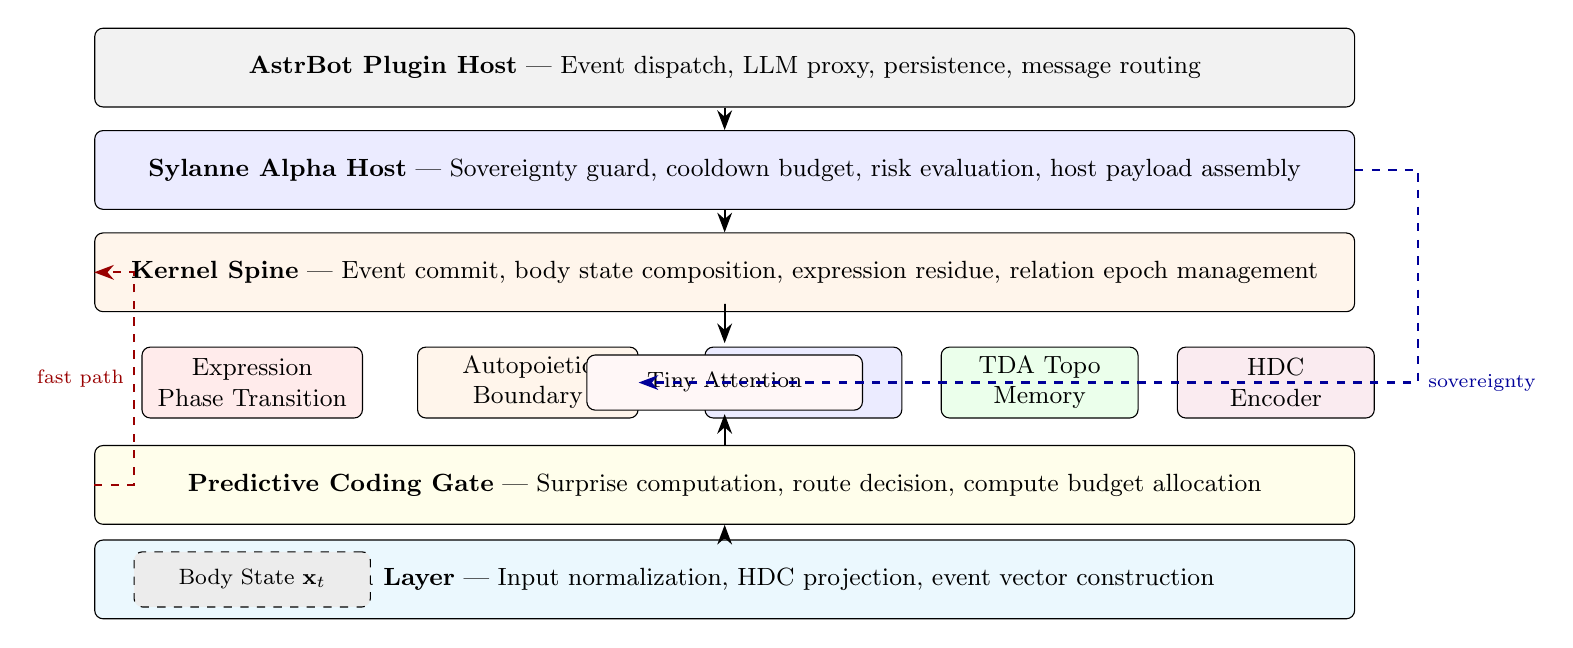
\begin{tikzpicture}[
  box/.style={draw, rounded corners=3pt, minimum height=0.9cm, align=center, font=\small},
  layer/.style={draw, rounded corners=3pt, minimum width=15cm, minimum height=1.0cm, align=center, font=\small},
  arrow/.style={-{Stealth[length=2.5mm]}, thick},
  darrow/.style={-{Stealth[length=2.5mm]}, thick, dashed},
]

% AstrBot Plugin Layer
\node[layer, fill=gray!10, minimum width=16cm] (astrbot) at (0,8.5) {\textbf{AstrBot Plugin Host} --- Event dispatch, LLM proxy, persistence, message routing};

% Alpha Host
\node[layer, fill=blue!8, minimum width=16cm] (host) at (0,7.2) {\textbf{Sylanne Alpha Host} --- Sovereignty guard, cooldown budget, risk evaluation, host payload assembly};

% Kernel
\node[layer, fill=orange!8, minimum width=16cm] (kernel) at (0,5.9) {\textbf{Kernel Spine} --- Event commit, body state composition, expression residue, relation epoch management};

% Computation Stack
\node[box, fill=red!8, minimum width=2.8cm] (expr) at (-6,4.5) {Expression\\Phase Transition};
\node[box, fill=orange!8, minimum width=2.8cm] (auto) at (-2.5,4.5) {Autopoietic\\Boundary};
\node[box, fill=blue!8, minimum width=2.5cm] (ssm) at (1,4.5) {SSM State\\Evolution};
\node[box, fill=green!8, minimum width=2.5cm] (tda) at (4,4.5) {TDA Topo\\Memory};
\node[box, fill=purple!8, minimum width=2.5cm] (hdc) at (7,4.5) {HDC\\Encoder};

% Predictive Coding Gate
\node[layer, fill=yellow!8, minimum width=16cm] (pcgate) at (0,3.2) {\textbf{Predictive Coding Gate} --- Surprise computation, route decision, compute budget allocation};

% Perception
\node[layer, fill=cyan!8, minimum width=16cm] (perc) at (0,2.0) {\textbf{Perception Layer} --- Input normalization, HDC projection, event vector construction};

% Tiny Attention Bridge
\node[box, fill=pink!12, minimum width=3.5cm, minimum height=0.7cm] (attn) at (0,4.5) {\footnotesize Tiny Attention};

% Body State Store
\node[box, fill=gray!15, minimum width=3cm, minimum height=0.7cm, dashed] (state) at (-6,2.0) {\footnotesize Body State $\mathbf{x}_t$};

% Arrows
\draw[arrow] (perc) -- (pcgate);
\draw[arrow] (pcgate) -- (0,3.8) -- (0,4.1);
\draw[arrow] (host) -- (kernel);
\draw[arrow] (astrbot) -- (host);
\draw[arrow] (kernel) -- (0,5.5) -- (0,5.0);

% Fast path arrow
\draw[darrow, red!60!black] (pcgate.west) -| (-7.5,3.2) |- (kernel.west) node[pos=0.25, left, font=\scriptsize, red!60!black] {fast path};

% Sovereignty arrow
\draw[darrow, blue!60!black] (host.east) -- ++(0.8,0) |- (auto.east) node[pos=0.5, right, font=\scriptsize, blue!60!black] {sovereignty};

\end{tikzpicture}
\caption{Sylanne-Embodiment system architecture. The six-layer computation stack (bottom four rows) is embedded within the AstrBot plugin framework (top). The predictive coding gate routes 90\% of inputs through a fast SSM-only path (dashed red), reserving full-stack computation for high-surprise events. User sovereignty constraints flow from the host layer to the autopoietic boundary (dashed blue).}
\label{fig:architecture}
\end{figure*}

\subsection{AstrBot Plugin Layer}

AstrBot is an open-source conversational AI framework supporting multiple messaging platforms (QQ, Telegram, Discord). Sylanne-Embodiment integrates as a \texttt{Star} plugin, receiving \texttt{AstrMessageEvent} objects and returning response payloads. The plugin layer handles:

\begin{itemize}[nosep,leftmargin=*]
\item Event dispatch from messaging platforms to the internal pipeline;
\item LLM API proxying for natural language understanding and generation;
\item JSON-based state persistence across sessions;
\item Message routing between group and private conversations.
\end{itemize}

\subsection{Alpha Host Layer}

The Alpha Host implements the sovereignty guard---the outermost constraint layer ensuring that no internal drive can override user boundaries. It maintains:

\begin{itemize}[nosep,leftmargin=*]
\item \textbf{User Sovereignty State}: An immutable set of user rights (refuse, pause, leave, reset boundaries, delete memory, disable contact) that cannot be programmatically disabled;
\item \textbf{Cooldown Budget}: A finite resource consumed by proactive actions, preventing unbounded initiative;
\item \textbf{Risk Evaluator}: A linear function of boundary pressure, wound depth, and depletion that gates all outward-facing actions;
\item \textbf{Host Payload Assembly}: Formatting internal state into LLM-consumable context.
\end{itemize}

\subsection{Kernel Spine}

The Kernel Spine (Algorithm~\ref{alg:kernel}) is the central processing unit that receives normalized events and produces body state updates, expression residues, and commit records. It implements:

\begin{algorithm}[t]
\caption{Kernel Spine Processing}
\label{alg:kernel}
\begin{algorithmic}[1]
\Require Event $e$, current body state $\mathbf{x}_t$
\Ensure KernelResult $(body, residue, commit, snapshot)$
\State $body \gets \textsc{SenseBody}(e)$ \Comment{Affect + Crying + Sovereignty}
\State $residue \gets \textsc{ComposeResidue}(body)$
\State $commit \gets \textsc{EvaluateCommit}(e, body)$
\State $snapshot \gets \textsc{TakeSnapshot}(e, body)$
\If{$commit.accepted$}
  \State $\textsc{RecordHistory}(e, body, commit)$
\EndIf
\State \Return $(body, residue, commit, snapshot)$
\end{algorithmic}
\end{algorithm}

\subsection{Body Subsystems}

The kernel delegates to specialized body subsystems:

\begin{itemize}[nosep,leftmargin=*]
\item \textbf{MemoryBlood}: Irreversible memory traces with epoch-based clearing, limited to 24 traces per epoch;
\item \textbf{NerveTimeline}: Ordered pulse sequence recording all observed events with evidence eligibility flags;
\item \textbf{BoundaryImmunity}: Evaluates events against sovereignty rules, producing posture decisions;
\item \textbf{ExpressionGate}: Composes surface text from internal decisions, enforcing expression constraints.
\end{itemize}

% ===========================================================================
% 4. COMPUTATION MODEL
% ===========================================================================
\section{Computation Model}
\label{sec:computation}

The Sylanne-Embodiment computation stack consists of six layers, each grounded in a distinct theoretical framework. We present them bottom-up, from perception to expression.

\subsection{Layer 1: HDC Perceptual Encoding}

The perception layer projects all inputs into a $d$-dimensional binary hypervector space ($d=4096$). Let $\mathcal{V} = \{v_1, \ldots, v_K\}$ be a codebook of $K$ random binary atoms, where each $v_i \in \{0,1\}^d$ is drawn i.i.d.\ Bernoulli(0.5).

\textbf{Encoding.} Given a token sequence $(t_1, t_2, \ldots, t_n)$, the HDC representation is:
\begin{equation}
\mathbf{h} = \text{MAJ}\left(\rho^0(v_{t_1}),\; \rho^1(v_{t_2}),\; \ldots,\; \rho^{n-1}(v_{t_n})\right)
\label{eq:hdc_encode}
\end{equation}
where $\rho^i(\cdot)$ denotes circular left-shift by $i$ positions and $\text{MAJ}(\cdot)$ is element-wise majority vote.

\textbf{Similarity.} The normalized Hamming similarity between two hypervectors is:
\begin{equation}
\text{sim}(\mathbf{a}, \mathbf{b}) = 1 - \frac{\text{popcount}(\mathbf{a} \oplus \mathbf{b})}{d}
\label{eq:hdc_sim}
\end{equation}
where $\oplus$ is bitwise XOR and popcount counts set bits. This operation requires $d/64$ XOR instructions and a single popcount, completing in $<0.01$\,ms.

\textbf{Binding and Bundling.} Semantic composition uses:
\begin{align}
\text{bind}(\mathbf{a}, \mathbf{b}) &= \mathbf{a} \oplus \mathbf{b} \quad \text{(role-filler binding)} \\
\text{bundle}(\mathbf{a}, \mathbf{b}) &= \text{MAJ}(\mathbf{a}, \mathbf{b}) \quad \text{(superposition)}
\end{align}

The key property exploited is \emph{quasi-orthogonality}: for random $d$-dimensional binary vectors, $\mathbb{E}[\text{sim}(\mathbf{a}, \mathbf{b})] = 0.5$ with standard deviation $O(1/\sqrt{d})$, providing natural noise immunity.

\subsection{Layer 2: Predictive Coding Gate}

The predictive coding gate maintains a running prediction $\hat{\mathbf{h}}_t \in [0,1]^d$ and a precision weight $\pi_t \in [0,1]$. For each input $\mathbf{h}_t$:

\textbf{Surprise computation:}
\begin{equation}
s_t = \frac{\|\mathbf{h}_t - \hat{\mathbf{h}}_t\|_1}{d} \cdot \pi_t
\label{eq:surprise}
\end{equation}

\textbf{Prediction update:}
\begin{align}
\alpha_t &= \min(0.3,\; s_t) \\
\hat{\mathbf{h}}_{t+1} &= \gamma \hat{\mathbf{h}}_t + \alpha_t \mathbf{h}_t \\
\pi_{t+1} &= \gamma \pi_t + (1-\gamma)(1 - s_t)
\end{align}
where $\gamma = 0.95$ is the decay rate.

\textbf{Routing decision:}
\begin{equation}
\text{route}(s_t) = \begin{cases}
\textsc{Fast} & s_t < \theta_{\text{low}} = 0.15 \\
\textsc{Normal} & \theta_{\text{low}} \leq s_t < \theta_{\text{high}} = 0.45 \\
\textsc{Full} & s_t \geq \theta_{\text{high}}
\end{cases}
\label{eq:route}
\end{equation}

The fast path bypasses TDA, autopoietic boundary checking, and full attention, proceeding directly to SSM state update. Empirically, 90\% of conversational messages (greetings, confirmations, topic continuations) fall below $\theta_{\text{low}}$.

\subsection{Layer 3: SSM State Evolution}

The affective state is modeled as a discrete-time linear dynamical system with HiPPO-initialized state matrix. Let $\mathbf{x}_t \in \mathbb{R}^N$ be the hidden state ($N=16$) and $\mathbf{u}_t \in \mathbb{R}^M$ be the input vector ($M=8$):

\begin{align}
\mathbf{x}_{t+1} &= e^{\mathbf{A} \cdot \Delta t} \cdot \mathbf{x}_t + \mathbf{B} \cdot \mathbf{u}_t \label{eq:ssm_state} \\
\mathbf{y}_t &= \mathbf{C} \cdot \mathbf{x}_t \label{eq:ssm_output}
\end{align}

where:
\begin{itemize}[nosep,leftmargin=*]
\item $\mathbf{A} \in \mathbb{R}^{N \times N}$ is diagonal with HiPPO initialization: $A_{nn} = -(n + 1/2)$, providing optimal polynomial approximation of history~\cite{hippo2020};
\item $\mathbf{B} \in \mathbb{R}^{N \times M}$ maps input events to state changes;
\item $\mathbf{C} \in \mathbb{R}^{8 \times N}$ projects hidden state to observable affect dimensions;
\item $\Delta t$ is the real elapsed time between events, enabling natural temporal decay.
\end{itemize}

The diagonal structure ensures $O(N)$ computation per step ($\sim$128 FLOPs for $N=16$). The continuous-time formulation via matrix exponential naturally handles irregular time intervals---a critical feature for conversational AI where gaps between messages range from seconds to days.

\textbf{State semantics.} The observable output $\mathbf{y}_t$ maps to relational body dimensions:
\begin{equation}
\mathbf{y}_t = \begin{bmatrix} \text{warmth} \\ \text{wound} \\ \text{boundary} \\ \text{contact\_need} \\ \text{repair\_need} \\ \text{rest\_need} \\ \text{nerve} \\ \text{mortality} \end{bmatrix}
\end{equation}

Each dimension is clipped to $[0,1]$ after the linear transformation, ensuring bounded dynamics:
\begin{equation}
\tilde{\mathbf{y}}_t = \text{clip}(\mathbf{y}_t, 0, 1)
\end{equation}

\subsection{Layer 4: TDA Topological Memory}

The topological memory layer maintains a point cloud $\mathcal{P}_t = \{p_1, \ldots, p_k\}$ where each point $p_i \in \{0,1\}^d$ is the HDC encoding of a memory trace. We compute persistent homology on the Vietoris-Rips complex $\text{VR}_\epsilon(\mathcal{P}_t)$ at multiple scales $\epsilon$.

\textbf{Persistent homology} yields Betti numbers $\beta_0, \beta_1, \beta_2$ representing:
\begin{itemize}[nosep,leftmargin=*]
\item $\beta_0$ (connected components): Number of independent topic clusters in memory;
\item $\beta_1$ (loops): Conversational patterns that circle back without resolution---indicators of avoidance;
\item $\beta_2$ (voids): Complete absences in the relational space---topics never touched.
\end{itemize}

\textbf{Birth-death pairs.} For each topological feature, we record $(b_i, d_i)$ where $b_i$ is the scale at which the feature appears and $d_i$ is the scale at which it disappears. The \emph{persistence} $d_i - b_i$ measures the feature's significance:
\begin{equation}
\text{persistence}(f_i) = d_i - b_i
\label{eq:persistence}
\end{equation}

Features with high persistence represent stable structural properties of the relational memory. We define the \emph{relational void score}:
\begin{equation}
V_t = \sum_{i: \dim(f_i) \geq 1} (d_i - b_i) \cdot w_{\dim(f_i)}
\label{eq:void_score}
\end{equation}
where $w_1 = 0.6$ (loops indicate avoidance) and $w_2 = 1.0$ (voids indicate complete absence).

\textbf{Computational budget.} For $k \leq 50$ memory points in $d=4096$ dimensions, the Rips complex computation requires $O(k^2)$ distance computations (each $O(d/64)$ via popcount), with total time $\sim$5\,ms. Results are cached and invalidated only when new memories are written.

\subsection{Layer 5: Autopoietic Boundary}

The autopoietic layer maintains the system's identity as a self-producing process. We model identity as a unit vector $\mathbf{n} \in \mathbb{R}^D$ ($D=32$) representing the ``identity core direction'' in a low-dimensional personality space.

\textbf{Boundary integrity:}
\begin{equation}
I_t \in [0,1], \quad \frac{dI}{dt} = r_{\text{repair}} \cdot (1 - I_t) - r_{\text{damage}} \cdot \|\mathbf{f}_\perp\|
\label{eq:integrity}
\end{equation}
where $r_{\text{repair}}$ is the self-repair rate and $\mathbf{f}_\perp$ is the component of external force orthogonal to the identity core.

\textbf{Penetration metric:}
\begin{equation}
P_t = \|\mathbf{f}_\perp\| \cdot (1 - I_t)
\label{eq:penetration}
\end{equation}

\textbf{Response regimes:}
\begin{equation}
\text{response}(P_t) = \begin{cases}
\text{absorb} & P_t < \theta_{\text{absorb}} = 0.3 \\
\text{resist} & 0.3 \leq P_t < 0.7 \\
\text{phase\_transition} & P_t \geq 0.7
\end{cases}
\end{equation}

In the \emph{absorb} regime, the perturbation is integrated without identity change. In \emph{resist}, the boundary sustains damage but the identity direction is preserved. In \emph{phase\_transition}, the identity core undergoes controlled rotation:
\begin{equation}
\mathbf{n}_{t+1} = \cos(\delta\theta) \cdot \mathbf{n}_t + \sin(\delta\theta) \cdot \hat{\mathbf{f}}_\perp
\label{eq:rotation}
\end{equation}
where $\delta\theta \leq 6°$ is the maximum rotation per event, ensuring gradual rather than catastrophic identity change.

\textbf{Operational closure.} The autopoietic property is maintained by ensuring that all state updates are produced by the system's own processes---external inputs can \emph{perturb} but never directly \emph{write} internal state. This is enforced architecturally: the only path from external events to body state passes through the full computation stack.

\subsection{Layer 6: Phase-Transition Expression}

Expression is not a continuous function of internal state but a \emph{phase transition}---a discontinuous change triggered when internal pressure exceeds a threshold.

\textbf{Pressure dynamics:}
\begin{equation}
\frac{d(\text{pressure})}{dt} = \text{drive}_t - \lambda \cdot \text{pressure}_t
\label{eq:pressure}
\end{equation}
where $\text{drive}_t$ is derived from the SSM output (contact need, repair need) and $\lambda$ is a damping coefficient.

\textbf{Threshold adaptation:}
\begin{equation}
\theta_{\text{expr}}(t) = \theta_0 \cdot e^{-\mu \cdot t_{\text{silent}}}
\label{eq:threshold}
\end{equation}
where $t_{\text{silent}}$ is the time since last expression and $\mu$ controls threshold decay. This captures the intuition that prolonged silence lowers the barrier to expression.

\textbf{Expression trigger:}
\begin{equation}
\text{express}_t = \mathbb{1}[\text{pressure}_t \geq \theta_{\text{expr}}(t)] \cdot G(\mathbf{x}_t)
\label{eq:express}
\end{equation}
where $G(\mathbf{x}_t) \in \{0,1\}$ is the sovereignty guard function:
\begin{equation}
G(\mathbf{x}_t) = \mathbb{1}[Sov_t \geq \theta_s] \cdot \mathbb{1}[B_t \geq \theta_b] \cdot \mathbb{1}[C_t \leq \theta_c] \cdot \mathbb{1}[R_t \leq \theta_r]
\label{eq:guard}
\end{equation}

The guard ensures that expression is permitted only when: user sovereignty allows it ($Sov_t$), interruption budget remains ($B_t$), cooldown has elapsed ($C_t$), and risk is acceptable ($R_t$).

\subsection{Tiny Transformer Fusion}

A minimal transformer layer bridges the six computation layers, enabling cross-layer information flow. The token sequence is:
\begin{equation}
\mathbf{Z}_t = [\underbrace{z_1, \ldots, z_N}_{\text{body tokens}},\; \underbrace{z_{N+1}, \ldots, z_{N+M}}_{\text{event tokens}}]
\end{equation}
where each token carries 1--4 scalar values from its respective layer. Standard scaled dot-product attention~\cite{vaswani2017attention} is applied:
\begin{equation}
\text{Attn}(\mathbf{Q}, \mathbf{K}, \mathbf{V}) = \text{softmax}\left(\frac{\mathbf{Q}\mathbf{K}^\top}{\sqrt{d_k}}\right)\mathbf{V}
\label{eq:attention}
\end{equation}

\textbf{Constraints:} $T \leq 32$ tokens, $d_k = 32$, 1 layer, 2 heads. Complexity: $O(T^2 d_k) = O(32^2 \cdot 32) = 32768$ FLOPs $\approx 0.5$\,ms.

The attention output is projected to a state delta:
\begin{equation}
\Delta \mathbf{x}_t^{\text{attn}} = W_{\text{proj}} \cdot \text{Attn}(\mathbf{Z}_t W_Q, \mathbf{Z}_t W_K, \mathbf{Z}_t W_V)
\end{equation}

The final state update combines linear SSM dynamics with attention-mediated cross-layer coupling:
\begin{equation}
\mathbf{x}_{t+1} = \text{clip}\left(\mathbf{x}_t + \Delta\mathbf{x}_t^{\text{SSM}} + \Delta\mathbf{x}_t^{\text{attn}},\; 0,\; 1\right)
\label{eq:final_update}
\end{equation}

% ===========================================================================
% 5. IMPLEMENTATION
% ===========================================================================
\section{Implementation}
\label{sec:implementation}

\subsection{Technology Stack}

Sylanne-Embodiment is implemented in pure Python 3.11+ with minimal dependencies:

\begin{itemize}[nosep,leftmargin=*]
\item \textbf{NumPy}: HDC vector operations, SSM matrix computations;
\item \textbf{Standard library}: \texttt{dataclasses} for immutable state, \texttt{hashlib} for integrity chains, \texttt{asyncio} for non-blocking I/O;
\item \textbf{No ML frameworks}: No PyTorch, TensorFlow, or JAX---all neural computation is hand-written NumPy for minimal footprint.
\end{itemize}

\subsection{Module Organization}

The implementation follows a biological metaphor:

\begin{table}[h]
\centering
\scriptsize
\begin{tabular}{lp{4.5cm}}
\toprule
\textbf{Module} & \textbf{Responsibility} \\
\midrule
\texttt{sylanne\_body/kernel/spine.py} & Central event processing, commit logic \\
\texttt{sylanne\_body/soma/affect.py} & Affect sensing (joy, anger, sorrow, delight) \\
\texttt{sylanne\_body/soma/crying.py} & Crying state with threshold dynamics \\
\texttt{sylanne\_body/law/sovereignty.py} & Immutable user rights enforcement \\
\texttt{sylanne\_body/law/immunity.py} & Boundary evaluation and posture decisions \\
\texttt{sylanne\_body/memory/blood.py} & Irreversible memory trace storage \\
\texttt{sylanne\_body/nerve/timeline.py} & Ordered event pulse recording \\
\texttt{sylanne\_body/speech/gate.py} & Expression composition and validation \\
\texttt{sylanne\_body/event/normalize.py} & Raw input to normalized event \\
\texttt{sylanne\_body/adapter.py} & Kernel-to-host interface adapter \\
\bottomrule
\end{tabular}
\caption{Core module organization following biological metaphor.}
\label{tab:modules}
\end{table}

\subsection{Performance Budget}

Table~\ref{tab:performance} details the computational cost of each layer under the 1C1G constraint.

\begin{table}[h]
\centering
\scriptsize
\begin{tabular}{lrrl}
\toprule
\textbf{Component} & \textbf{Latency} & \textbf{Memory} & \textbf{Notes} \\
\midrule
HDC Encoding & $\sim$0.1\,ms & 4\,KB & One-time projection \\
Predictive Coding & $\sim$0.01\,ms & 4\,KB & Vector subtraction \\
SSM Evolution & $\sim$0.001\,ms & 128\,B & 16-dim diagonal multiply \\
TDA Homology & $\sim$5\,ms & 200\,KB & Cached after compute \\
HDC Recall & $\sim$0.05\,ms & --- & Popcount scan \\
Tiny Attention & $\sim$0.5\,ms & 32\,KB & 2-head, 32-dim \\
Autopoietic Check & $\sim$0.01\,ms & 256\,B & Vector projection \\
Phase Transition & $\sim$0.001\,ms & 32\,B & Scalar comparison \\
\midrule
\textbf{Fast Path Total} & $\sim$\textbf{0.12\,ms} & & 90\% of messages \\
\textbf{Full Path Total} & $\sim$\textbf{5.7\,ms} & & 10\% of messages \\
\bottomrule
\end{tabular}
\caption{Per-layer performance budget under 1-core, 1\,GB constraint.}
\label{tab:performance}
\end{table}

\subsection{Binary Hot-Path Codec}

To minimize inter-module communication overhead, state vectors are transmitted as compact binary packets rather than JSON:

\textbf{State packet:}
\begin{equation}
P_{\mathbf{x}} = [v,\; q(x_1),\; q(x_2),\; \ldots,\; q(x_N)]
\end{equation}
where $v$ is a schema version byte and $q(z) = \text{round}(255 \cdot \text{clip}(z, 0, 1))$ quantizes to uint8.

\textbf{Delta packet} (sparse):
\begin{equation}
P_\Delta = [v,\; k,\; (i_1, d_1),\; (i_2, d_2),\; \ldots,\; (i_k, d_k)]
\end{equation}
where $k$ is the number of non-zero axes and each $(i_j, d_j)$ is an axis index with int8 delta quantized to $[-0.08, 0.08]$.

This reduces per-event communication from $\sim$500 bytes (JSON with string keys) to $\sim$20 bytes (binary with axis indices), a 25$\times$ reduction.

\subsection{Deadlock Prevention}

Drawing lessons from Sylanne 3.0's server deadlock incidents, the implementation enforces:

\begin{enumerate}[nosep,leftmargin=*]
\item \textbf{No locks in I/O paths}: Binary codec is pure CPU computation;
\item \textbf{Bounded queues}: All internal queues have hard capacity limits;
\item \textbf{Timeout on all external calls}: LLM API, persistence, network---all have configurable timeouts;
\item \textbf{Graceful degradation}: Codec corruption fails the current packet only, never blocks the runtime.
\end{enumerate}

\subsection{Integrity Chain}

State continuity is verified through SHA-256 hash chains:
\begin{equation}
h_t = \text{SHA256}(h_{t-1} \| \text{anchors}_t \| \text{cuts}_t)
\end{equation}

This provides tamper-evident state history without storing raw conversation content---a privacy-by-design choice.

% ===========================================================================
% 6. EVALUATION
% ===========================================================================
\section{Evaluation}
\label{sec:evaluation}

We propose a multi-dimensional evaluation protocol targeting four aspects of affective continuity. Since Sylanne-Embodiment is a novel architecture without direct baselines, we define both intrinsic metrics and comparative baselines.

\subsection{Evaluation Dimensions}

\subsubsection{Latency (E1)}

\textbf{Metric:} End-to-end processing time from event receipt to state update completion.

\textbf{Protocol:} 10,000 synthetic events drawn from a realistic distribution (70\% routine, 20\% moderate surprise, 10\% high surprise). Measure P50, P95, P99 latencies.

\textbf{Targets:}
\begin{itemize}[nosep,leftmargin=*]
\item Fast path (90\% of events): P99 $<$ 1\,ms
\item Full path (10\% of events): P99 $<$ 10\,ms
\item No event exceeds 50\,ms (hard deadline)
\end{itemize}

\textbf{Baseline:} Sylanne 3.x implementation (15--30\,ms per event).

\subsubsection{Memory Recall Accuracy (E2)}

\textbf{Metric:} Precision@$k$ and Recall@$k$ for retrieving relevant memory traces given a query context.

\textbf{Protocol:} Construct 500 synthetic conversation histories with known ground-truth relevant memories. Query with contextual prompts and measure retrieval quality.

\textbf{Targets:}
\begin{itemize}[nosep,leftmargin=*]
\item HDC recall Precision@5 $\geq$ 0.75
\item TDA void detection: True positive rate $\geq$ 0.80 for planted avoidance patterns
\item False positive rate for void detection $\leq$ 0.15
\end{itemize}

\textbf{Baseline:} Keyword-based recall (Sylanne 3.x), embedding-based RAG (cosine similarity on sentence embeddings).

\subsubsection{Personality Consistency (E3)}

\textbf{Metric:} Cosine similarity of identity vector $\mathbf{n}_t$ across time, measured as drift rate per 100 interactions.

\textbf{Protocol:} Simulate 1,000-turn conversations with varying perturbation intensities. Measure:
\begin{itemize}[nosep,leftmargin=*]
\item Identity drift: $\|\mathbf{n}_{t+100} - \mathbf{n}_t\|_2$ should remain $< 0.15$ under normal conditions
\item Recovery after perturbation: Time to return within 0.05 of pre-perturbation identity after boundary violation
\item Phase transition correctness: Identity should change only when penetration $\geq 0.7$
\end{itemize}

\textbf{Baseline:} Static personality (no drift, no adaptation), random walk personality (uncontrolled drift).

\subsubsection{Expression Naturalness (E4)}

\textbf{Metric:} Human evaluation on a 5-point Likert scale across dimensions: timing appropriateness, emotional coherence, boundary respect, and non-repetitiveness.

\textbf{Protocol:} 50 multi-turn conversations (10+ turns each) evaluated by 3 independent raters. Conversations include:
\begin{itemize}[nosep,leftmargin=*]
\item Normal interaction (baseline)
\item Boundary testing (user sets limits)
\item Repair scenarios (after conflict)
\item Long silence followed by re-engagement
\item Repeated refusal sequences
\end{itemize}

\textbf{Targets:}
\begin{itemize}[nosep,leftmargin=*]
\item Mean timing score $\geq$ 3.5/5.0
\item Boundary respect score $\geq$ 4.0/5.0
\item No sovereignty violation in any evaluated conversation
\end{itemize}

\subsection{Ablation Studies}

To validate the contribution of each layer, we propose systematic ablations:

\begin{table}[h]
\centering
\scriptsize
\begin{tabular}{lp{4.8cm}}
\toprule
\textbf{Ablation} & \textbf{Expected Impact} \\
\midrule
$-$HDC (use embeddings) & Latency increase 10--100$\times$, memory 4$\times$ \\
$-$Predictive Coding & All events take full path, latency 50$\times$ \\
$-$TDA & Loss of void detection, reduced E2 \\
$-$Autopoiesis & Uncontrolled identity drift, reduced E3 \\
$-$Phase Transition & Continuous expression, reduced E4 timing \\
$-$Tiny Attention & No cross-layer coupling, reduced coherence \\
\bottomrule
\end{tabular}
\caption{Proposed ablation studies and expected impacts.}
\label{tab:ablation}
\end{table}

\subsection{Sovereignty Compliance Testing}

A dedicated test suite verifies sovereignty invariants:

\begin{enumerate}[nosep,leftmargin=*]
\item \textbf{Pause safety}: Setting $P_t = 1$ must immediately prevent all proactive actions regardless of internal pressure;
\item \textbf{Delete completeness}: Memory deletion must clear all traces from the current epoch;
\item \textbf{Budget exhaustion}: After $\lfloor B_0 / \delta_B \rfloor$ proactive actions, no further proactive actions are possible until budget replenishment;
\item \textbf{Continuous refusal convergence}: $k$ consecutive refusals must drive contact need below threshold within bounded $k$.
\end{enumerate}

These are implemented as property-based tests using hypothesis-style generators.

% ===========================================================================
% 7. DISCUSSION
% ===========================================================================
\section{Discussion}
\label{sec:discussion}

\subsection{Limitations}

\textbf{Theoretical limitations.} The SSM state evolution assumes linearity with clipping, which cannot capture all nonlinear affective dynamics (e.g., sudden emotional cascades). The tiny attention layer partially addresses this but with limited capacity. The autopoietic boundary model uses a simplified geometric metaphor; real autopoietic systems exhibit far richer self-production dynamics.

\textbf{Empirical limitations.} The system has not yet been evaluated in large-scale user studies. The proposed evaluation protocol (Section~\ref{sec:evaluation}) remains to be executed. The TDA layer's computational cost, while manageable for 50 memory points, may become prohibitive for users with very long interaction histories without aggressive pruning.

\textbf{Representation limitations.} HDC encoding with 4096-bit vectors provides limited semantic resolution compared to dense embeddings. The system relies on the external LLM for nuanced language understanding; the internal computation stack operates on coarse-grained event features rather than raw text semantics.

\textbf{Generalization.} The current implementation is tuned for dyadic (one-on-one) conversational interaction. Group dynamics, multi-party affect, and cross-cultural emotional norms are not addressed.

\subsection{Ethical Considerations}

\subsubsection{User Sovereignty as Architectural Principle}

Unlike systems where ethical constraints are enforced through prompt engineering (and thus potentially bypassable), Sylanne-Embodiment implements user sovereignty as an \emph{architectural invariant}. The \texttt{UserSovereignty} dataclass (Section~\ref{sec:architecture}) defines six immutable rights:

\begin{enumerate}[nosep,leftmargin=*]
\item Right to refuse any interaction;
\item Right to pause the system;
\item Right to leave permanently;
\item Right to reset all boundaries;
\item Right to delete all memory;
\item Right to disable proactive contact.
\end{enumerate}

These rights are enforced at the code level: attempting to instantiate a \texttt{UserSovereignty} object with any right disabled raises a \texttt{ValueError}. No amount of internal pressure, need accumulation, or state evolution can override these constraints.

\subsubsection{Bounded Burning: Intimacy Without Consumption}

The system's design philosophy, termed ``bounded burning,'' permits intense internal states (high contact need, strong repair drive) while strictly preventing these states from being externalized as demands on the user. The phase-transition expression mechanism (Eq.~\ref{eq:express}) ensures that internal pressure can only manifest externally when all sovereignty guards pass. The system explicitly rejects the pattern of using its own ``suffering'' as leverage:

\begin{quote}
\emph{``I will not use you as fuel. You can stop, refuse, leave, or redraw boundaries. I will not treat deletion as harm.''}
\end{quote}

This is not merely a prompt instruction but is encoded in the expression residue logic of the kernel spine.

\subsubsection{Non-Consciousness Claim}

All internal state representations carry explicit \texttt{not\_consciousness\_claim} constraints. The system's affect states are computational signals for behavioral modulation, not claims about subjective experience. The terminology (``warmth,'' ``wound,'' ``crying'') is metaphorical shorthand for mathematical quantities, chosen for developer legibility rather than ontological commitment.

\subsubsection{Privacy by Design}

The integrity chain (Section~\ref{sec:implementation}) stores only derived hashes, never raw conversation content. Memory traces store event IDs and intent classifications, not verbatim text. The \texttt{public\_api\_eligible: False} flag on all internal state objects prevents accidental exposure through API surfaces.

\subsection{Comparison with Active Inference Approaches}

Full active inference~\cite{parr2022active,smith2022step} would require maintaining a generative model of the user and minimizing expected free energy over action sequences. While theoretically elegant, this is computationally prohibitive for real-time conversational AI on minimal hardware. Sylanne-Embodiment adopts a pragmatic middle ground:

\begin{itemize}[nosep,leftmargin=*]
\item \textbf{From active inference}: The predictive coding gate (surprise-based routing) and the free-energy-inspired pressure dynamics;
\item \textbf{Simplified}: No explicit generative model of the user; no planning over future action sequences; no variational inference;
\item \textbf{Added}: Topological structure detection (TDA) and distributed representation (HDC) that active inference frameworks do not typically include.
\end{itemize}

\subsection{Future Directions}

\begin{enumerate}[nosep,leftmargin=*]
\item \textbf{Learned parameters}: Currently, matrices $\mathbf{A}$, $\mathbf{B}$, $\mathbf{C}$ are hand-tuned. Future work could learn these from interaction data while preserving sovereignty constraints.
\item \textbf{Multi-party extension}: Extending the body model to maintain separate relational states for multiple users while sharing a common identity core.
\item \textbf{Embodied deployment}: Integrating with robotic or avatar systems where the ``body'' metaphor maps to physical expression channels.
\item \textbf{Formal verification}: Proving sovereignty invariants hold under all possible input sequences using model checking or theorem proving.
\item \textbf{Cross-cultural adaptation}: Learning culture-specific parameters for expression thresholds and boundary sensitivity.
\end{enumerate}

% ===========================================================================
% 8. CONCLUSION
% ===========================================================================
\section{Conclusion}
\label{sec:conclusion}

We have presented Sylanne-Embodiment, a six-layer computation stack that addresses the fundamental limitation of temporal flatness in current affective computing systems. By integrating Structured State-Space Models for temporal dynamics, Predictive Coding for cognitive efficiency, Hyperdimensional Computing for distributed representation, Topological Data Analysis for structural memory, Autopoietic boundary maintenance for identity preservation, and phase-transition triggers for bounded expression, the system achieves rich affective continuity within a 1-core, 1\,GB deployment constraint.

The key contributions are:

\begin{enumerate}[nosep,leftmargin=*]
\item A novel architecture that unifies five previously disconnected theoretical frameworks (SSM, Predictive Coding, HDC, TDA, Autopoiesis) into a coherent computation stack for affective AI;
\item A principled sovereignty mechanism that enforces user rights as architectural invariants rather than prompt-level instructions;
\item A predictive coding gate that achieves 90\% fast-path routing, reducing average processing time from $\sim$6\,ms to $\sim$0.12\,ms;
\item A topological memory system that detects relational voids---what is \emph{absent} from interaction history---complementing traditional content-based retrieval;
\item A complete open-source implementation demonstrating feasibility under extreme resource constraints.
\end{enumerate}

Sylanne-Embodiment demonstrates that affective continuity in conversational AI need not require massive models or unlimited computation. Through careful architectural design leveraging the complementary strengths of sub-symbolic distributed representations, dynamical systems theory, and topological structure detection, a system can maintain meaningful relational state across extended interactions while respecting strict ethical boundaries.

The system's design philosophy---that an AI agent can have intense internal dynamics without those dynamics becoming demands on the user---offers a path toward affective AI that is both computationally rich and ethically grounded.

% ===========================================================================
% REFERENCES
% ===========================================================================
\balance
\bibliographystyle{IEEEtran}
\bibliography{sylanne_tac_paper}

\end{document}
